\chapter{Methodology}
\section{S1 Handover in srsRAN}
\begin{itemize}
    \item Understanding the effects of indoor handover requires the use of a software stack
    \item Most mobile operators use a proprietary stack, very little of which is available to the general public or researchers
    \item srsRAN is an open-source mobile network stack developed for both commercial use and research
\subsection{ZMQ-based Handover}
    \item Following \cite{powell_handover_2021}, I started with a pure simulation-based experiment of inducing an S1 handover
    \item This is accomplished by using ZMQ and GNU Radio to simulate the radio layer.
    \item We set up the experiment by running an Open5gs network core, two srsENBs and a srsUE
    \item The eNBs are connected to the network core over the S1AP interface over TCP on my local machine
    \item The eNBs were both connected to the UE using GNU radio and ZMQ, communicating over various TCP ports.
    \item To emulate propagation loss, we add multiply blocks on both connections (send and receive) from UE to each eNB, initially setting it to 1 for the eNB we designate as the source cell and 0 for the "target" cell
    \item On the srsUE process, we collect the measurement logs, fetching the RSRP for both cells
    \item We gradually increase the multiply for the target cell, until the UE is handed over to the target cell
    \item Figure \ref{fig:methods:zmq-s1-handover} shows the results of said experiment
    \item As the handover is triggered by default using the A3 Event Trigger, we can see that the A3 offset used in our configuration was 3dBm.
    \item On a static source analysis of the srsRAN code we see the handover occurs when the following condition is met:
$$\text{RSRP}_\text{Target} - \text{RSRP}_\text{Source} > \text{Hysteresis} + \text{A3 Offset} + \text{Of} + \text{Oc}$$
where 
$$\begin{aligned}\text{Of} &= \text{Frequency Offset}_\text{Target} - \text{Frequency Offset}_\text{Source} \\
\text{Oc} &= \text{Cell Offset}_\text{Target} - \text{Cell Offset}_\text{Source}\end{aligned}$$
for the default setup, $\text{Of}=0$ and $\text{Oc}=0$
\item Furthermore Hysteresis is set to 0, and in our configuration, A3 Offset was set to 3dBm, and so we see srsRAN behaving as expected according to the LTE specification.
\end{itemize}
\begin{figure}
    \centering
    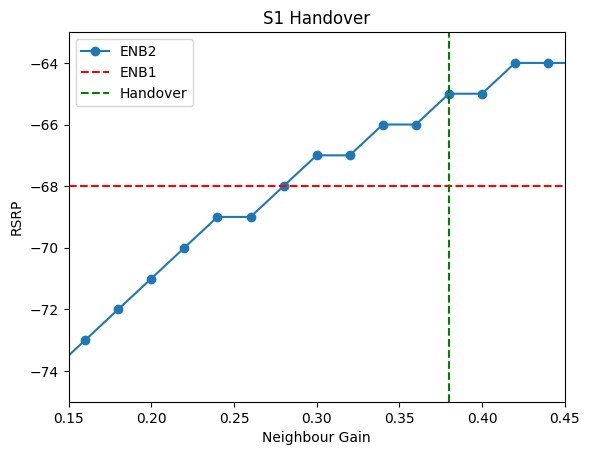
\includegraphics[width=1\linewidth]{src/img/zmq_s1_handover.png}
    \caption{S1 Handover occurring in srsRAN with simulated UE over ZMQ/GNU Radio}
    \label{fig:methods:zmq-s1-handover}
\end{figure}
\section{Custom Network Simulator}
\begin{itemize}
    \item We look at \cite{hatipoglu_handover-based_2020} to better understand how large scale handovers are conducted
    \item We replicate their findings, to understand what causes ping pong
    \item Propagation loss was modelled with path shadow loss
    \item As the authors did not release the tool they built, we reconstructed the tool, as seen in Figure \ref{fig:methods:grouped-uesim}
\begin{figure}
    \centering
    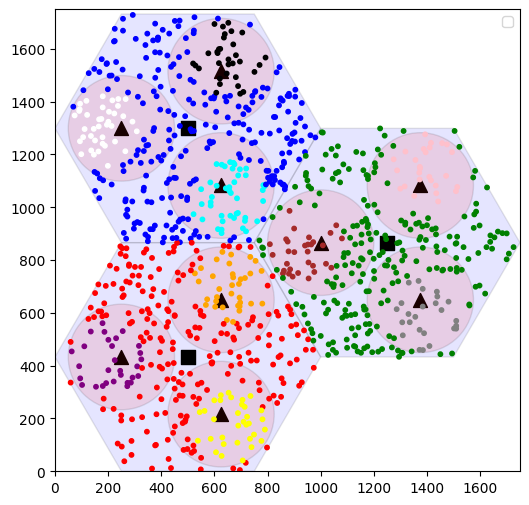
\includegraphics[width=0.75\linewidth]{src//img/grouped_uesim.png}
    \caption{An overview of the 2D simulator}
    \label{fig:methods:grouped-uesim}
\end{figure}
\subsection{Understating Ping Pong Handover}
\item We run the experiment with various handover parameters in Figure \ref{fig:methods:pingpong-uesim}:
\begin{figure}
    \centering
    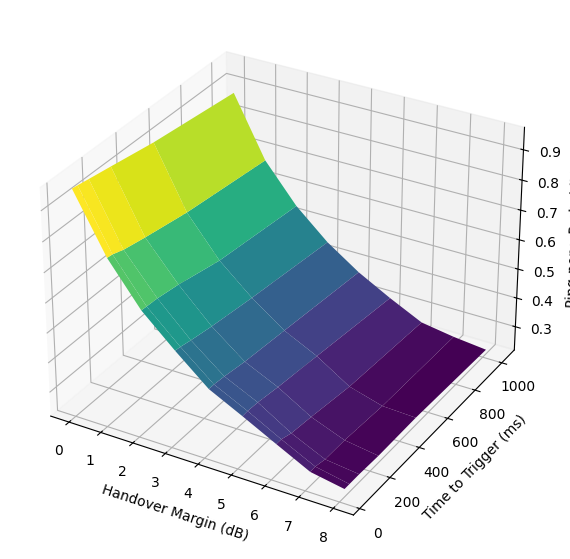
\includegraphics[width=0.5\linewidth]{src//img/pingpong_uesim.png}
    \caption{Ping Pong vs Hysteresis and TTT}
    \label{fig:methods:pingpong-uesim}
\end{figure}
\end{itemize}

\section{Network Testbed}
\begin{itemize}
    \item After performing the initial experiments in a simulator, we move onto testing in the real world
    \item The testbed consists of 4 NUCs, each connected to a Ettus Research B210 USRP. 
    \item Each NUC runs a modified srsENB process, enabled with an E2 RIC interface to be oRAN compatible. 
    \item Open5gs is running on another server, and is connected using the S1 interface
    \item The entire setup is orchestrated using KOperators \todo{find citation}, a Kubernetes deployment framework for ORAN.
\end{itemize}

\subsection{Handover with 2 eNBs }
\begin{itemize}
    \item We enable two of the eNBs, and run srsUE on an external machine also attached with a B210 USRP
    \item The logs of the UE are saved to disk, with RRC logs set to DEBUG
\end{itemize}

\subsubsection{Experiment: Walk from Source to Target and Back}
\begin{itemize}
    \item The first experiment ran was a trivial situation of walking from one eNB to another and back again
    \item We expect that the RSRP of each eNB will be proportional to the distance to the UE
    \item We expect the RSRP of the target cell to rise and the source to lower as we approach the target, and vice versa as we return. 
    \item We expect a handover event to occur just past the halfway mark, and another on the way back
    \item Figure \ref{fig:methods:2024-02-09-multi-ho} shows the RSRP and the connected cell for the experiment
\begin{figure}
    \centering
    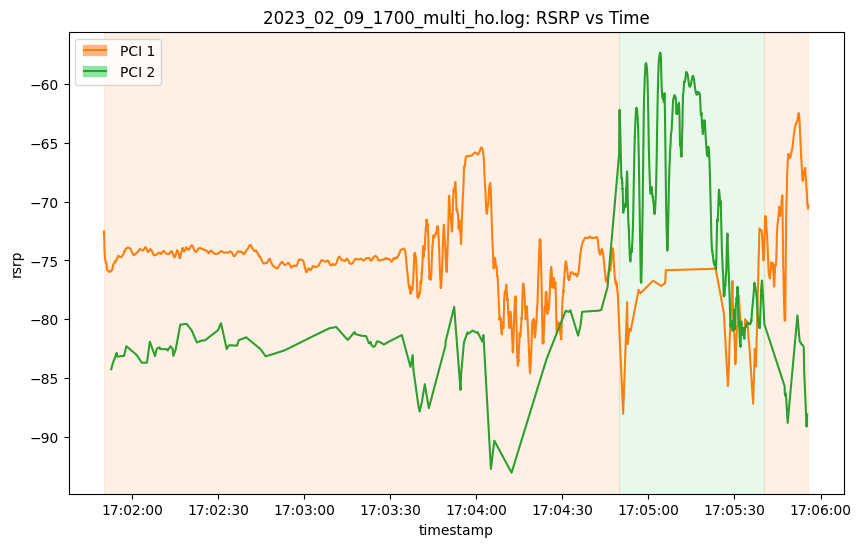
\includegraphics[width=0.75\linewidth]{src//img/2024_02_09_multiho.png}
    \caption{RSRP and Connected Cell for a walking back and forth episode}
    \label{fig:methods:2024-02-09-multi-ho}
\end{figure}

\item We see the expected outcome, however with much more noise than expected
\item To test the impact the extent of the noise, we perform another experiment
\end{itemize}

\subsubsection{No Movement}
\begin{itemize}
    \item To determine the extent of background noise, we setup the experiment similarly to the previous, but with the UE set in the centre of the room
    \item We start the UE and after a period of movement, it remains still
    \item We see in Figure \ref{fig:methods:2024-02-09-wait}

\begin{figure}
    \centering
    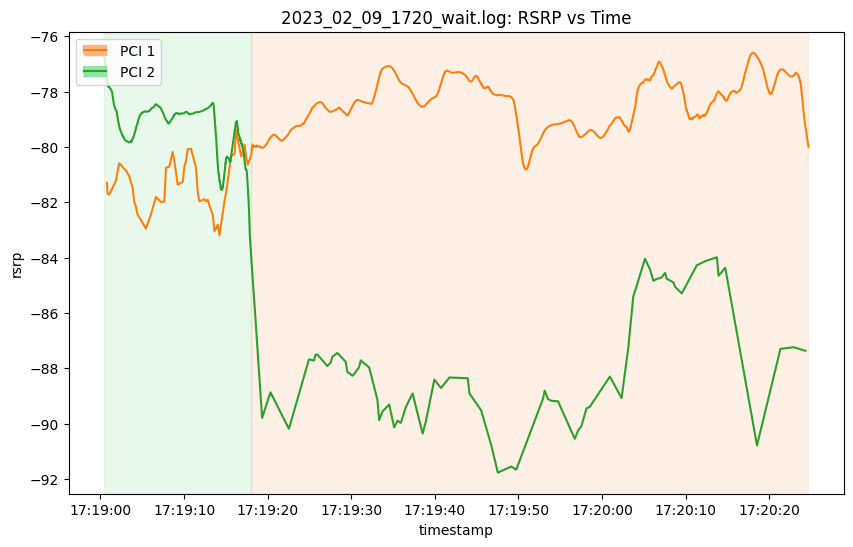
\includegraphics[width=0.75\linewidth]{src//img/2024_02_09_wait.png}
    \caption{2 eNB, no movement}
    \label{fig:methods:2024-02-09-wait}
\end{figure}

    \item Even with no movement, there are very large spikes in RSRP for both UEs
    \item This could have very large impacts on Ping Pong Rates
    \item To accentuate these results, we perform the same experiment, but with slowly rotating the UE back and forth
\end{itemize}

\subsubsection{Rotating UE}
\begin{itemize}
    \item We put the UE in the centre of the room
    \item We rotate the UE back and forth
    \item The results are in Figure \ref{fig:methods:2024-02-09-rotate}
    \begin{figure}
        \centering
        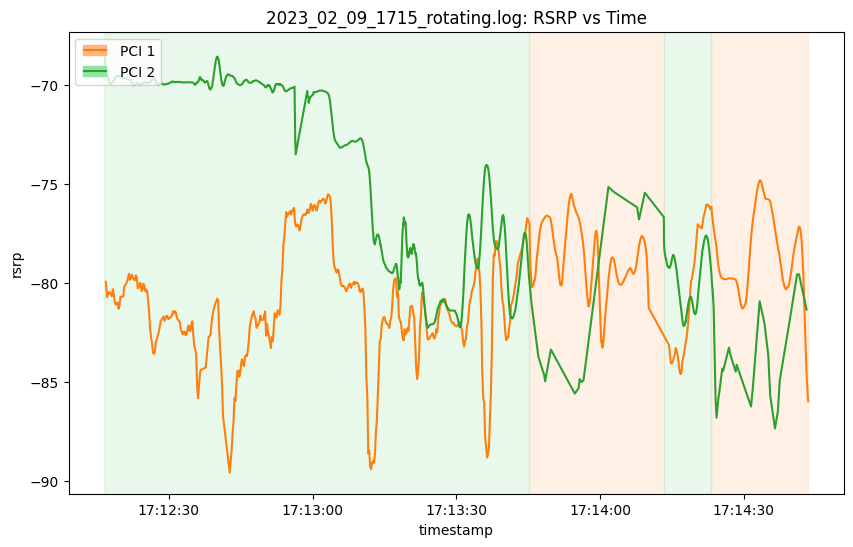
\includegraphics[width=0.75\linewidth]{src//img/2024_02_09_rotating.png}
        \caption{Rotating UE}
        \label{fig:methods:2024-02-09-rotate}
    \end{figure}
    \item We see a much higher incidence of handover occurring
\end{itemize}

\subsubsection{LOS Blockage}
\begin{itemize}
    \item We perform the same setup as the waiting one, but instead of remaining stationary, we intentionally walking in front of the UE to emulate people moving around in a room
    \item Results in Figure \ref{fig:methods:2024-02-09-walking}
\begin{figure}
    \centering
    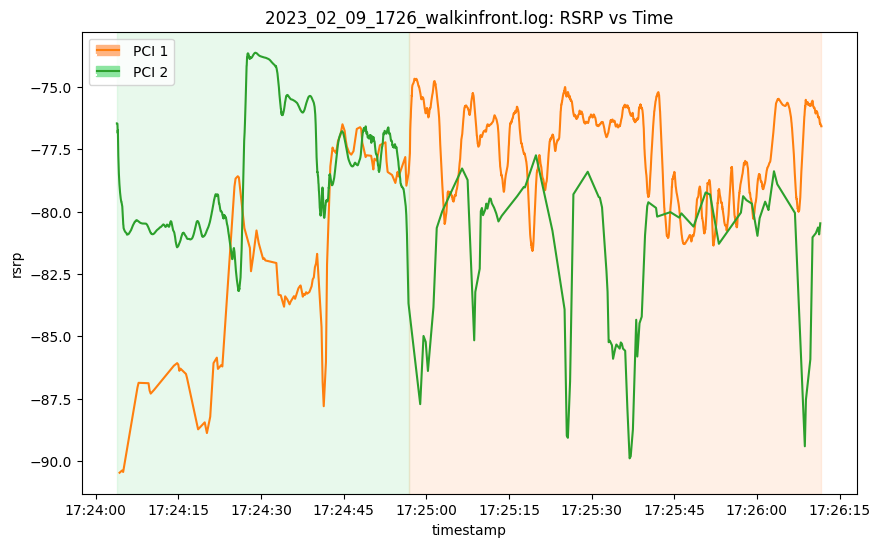
\includegraphics[width=0.75\linewidth]{src//img/2024_02_09_los_block.png}
    \caption{LOS Blockage by walking around}
    \label{fig:methods:2024-02-09-walking}
\end{figure}

\item We see higher than expected spikes in RSRP caused by the walking, many of which are higher than the 3dBm need to trigger handover
\item \end{itemize}